\section{Design Choices}

Some of the primary design choices in the project are summarized below:

\subsection{Choice of Scala as Host Language}
\textbf{Choice of Scala as host language}: The adoption of Scala has grown tremendously over the last 5 years in the industry with large organizations such as Twitter, Bank of America Merrill Lynch and Groupon using it for DSL design \cite{scala}. The expressive syntax and intelligent type inference allows a clean domain syntax and type system to be developed. Portability of code because of the JVM platform is another factor promoting Scala's adoption \cite{scala}. The reasons for using Scala are summarized below:

\begin{figure}[H]
  \centering
    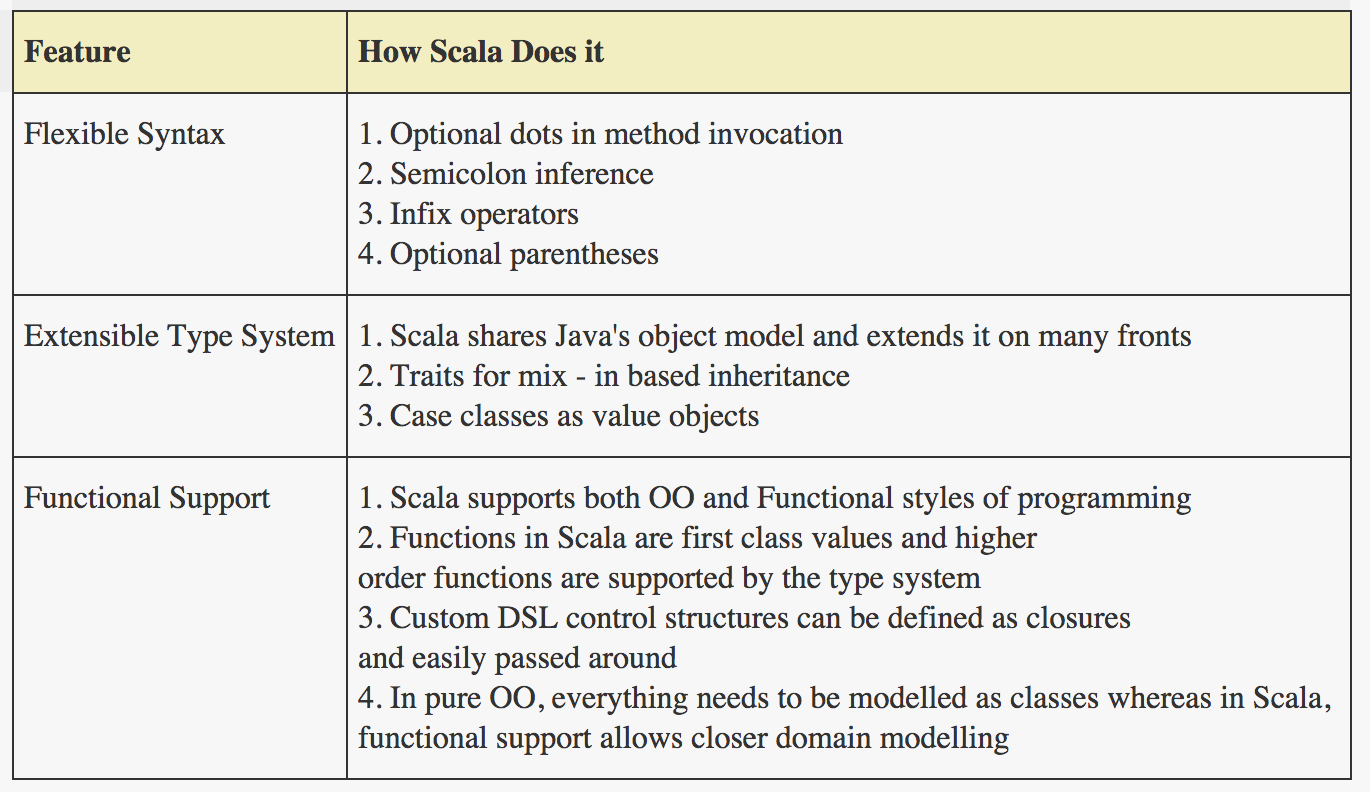
\includegraphics[width=500px]{figures/scala_motivation.png}
  \caption{Motivation for using Scala}
\end{figure}

\subsection{Comparison of Scala and Python for DSL implementation}

The reporting DSL was developed in both Scala and Python to assess the trade - offs. The functionality desired in the DSL was:
\begin{itemize}
\item Check out different commits for a particular \textbf{mercurial} branch
\item Check out different branches for a particular \textit{mercurial} repository
\item Ease of configuring system and ability to hot - switch settings during run - time
\item \textbf{Object Orientation} for readability and maintainability
\item Ability to run tests on all branches/commits and report results reliably
\end{itemize}

\noindent
\textbf{Dynamic languages}, such as Python, Ruby, Dylan, LISP, Scheme, and Smalltalk, are languages designed to increase programmer efficiency. Dynamic
languages enables faster development cycles by allowing parts of a program to be modified at run time. Functions may be introduced, removed, or changed, classes added, class inheritance modified, and modules can be created or removed. This allows a programmer to quickly test a new feature, or a new piece of code. Furthermore, modern dynamic languages, such as Python and Ruby, provide syntax and high-level programming models that are easy to learn, resulting in higher productivity \cite{lund}.
\bigskip

\subsubsection{Scala vs.Python Advantages}
\noindent
Some of the advantages of Python over Scala were:
\begin{itemize}
\item Dynamic Language
\item Support for scripting
\item Lower development time
\end{itemize}

\noindent
Some of the advantages of Scala over Python were:
\begin{itemize}
\item Greater type safety due to compile time checking
\item Better collections hierarchy
\item Expressiveness
\item High readability
\end{itemize}

\subsubsection{Conclusion - Scala is more suitable for DSL development}

\begin{figure}[H]
  \centering
    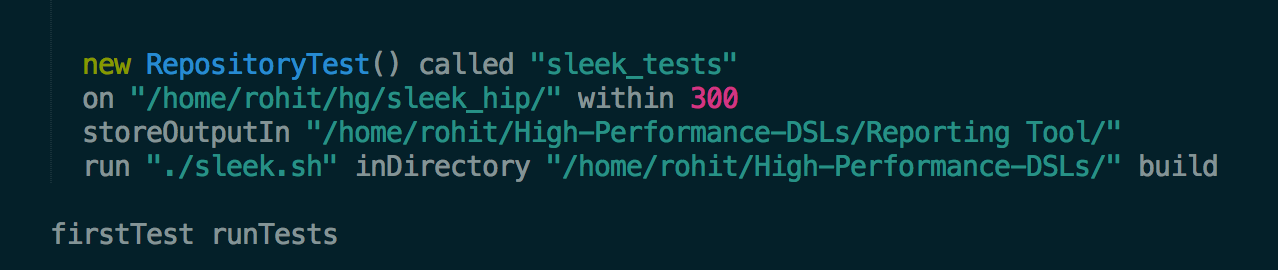
\includegraphics[width=500px]{figures/reportingDSL.png}
  \caption{Reporting DSL syntax}
\end{figure}

\noindent
Overall, \textbf{Scala} was concluded to be more suitable for DSL development. The primary reason for this was \textit{type - safety}. DSLs can grow to several tens of thousands of lines of code and type - safety makes development a lot more robust and secure.

\subsection{Choice of Embedded DSL Approach}
Instead of starting off development using the Delite Framework or the Lightweight Modular Staging Library, I decided to write a DSL with an embedded type system and no run - time code generation or optimizations. This allowed me to understand the important types and constructs required in the domain and develop a clean syntax. It also allowed me to model the domain without concerning myself with lower level optimizations prematurely. Some of the advantages of creating an embedded DSL were:
\begin{itemize}
\item \textbf{Lightweight} - The DSL has been written as a \textit{library} which can be easily included in other projects by simply adding the .JAR file to the project build path.
\item \textbf{Compile time type checking} - Since there is no code generated at run - time or any meta - programming, all types are checked at compile - time giving us the added support of the Scala compiler.
\item \textbf{Easily maintainable and extensible} - Since the source code is written using the Scala language, it is readable and easily extensible if new functionality is desired. The system also follows the \textbf{open - closed} principle. It is open for extension but closed for modification.
\item \textbf{Emphasis on Semantics} - Domain rules can vary and can require extension or revision. It is very important that the DSL provides \textit{Pluggable semantics} according to Ghosh \cite{dslsInAction}. Appropriate usage of Scala types including \textit{traits, types and objects} make the semantics quite meaningful. For example, when we want to add a test, we can write syntax like:

\begin{figure}[H]
  \centering
    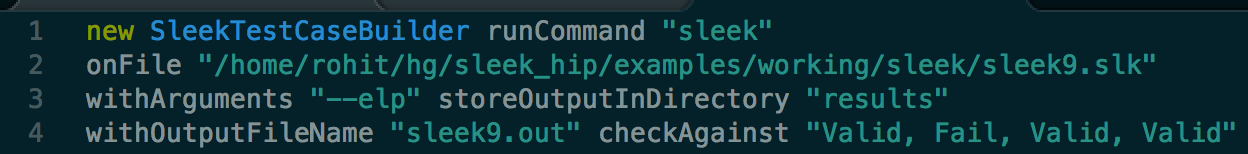
\includegraphics[height=60px]{figures/declarative_syntax.png}
  \caption{Meaningful Semantics}
\end{figure}

\item \textbf{Loose Coupling} - Loose coupling between the composed DSLs, and their rules, allowing all the rules to evolve independently.
\item \textbf{Representation Independence} - The DSL does not contain any embedded implementation details and merely shows domain abstractions.
\end{itemize}

\newpage
\subsection{Design Patterns}

Design pattern are well known solutions for recurring problems. By defining and categorizing patterns, a catalog of patterns can be created for use when building large and complex software systems \cite{gof}. Ghosh \cite{dslsInAction} talks about certain design patterns being industry "best - practices" for DSL development. Over the course of this project, these patterns have been used extensively.
\bigskip

\noindent
There are several benefits of using design patterns. Patterns are known solutions for building software systems. This helps increase maintainability, extensibility and readability of the code base \cite{iceland}.

\subsubsection{Singleton Pattern}
The singleton pattern restricts the instantiation of a class to one object, and provides a global point of access to \cite{gof}. It is used when the developer does not want multiple implementations of the type in heap memory. Pure functions, file - system utilities are some of the methods we can wrap inside Utility objects. In this project, the singleton has been used for re - usable components like regular expression and file system utilities. Scala provides an \textbf{Object} type that implements this pattern without requiring any boilerplate code. An example of this pattern is shown below:

\begin{figure}[H]
  \centering
    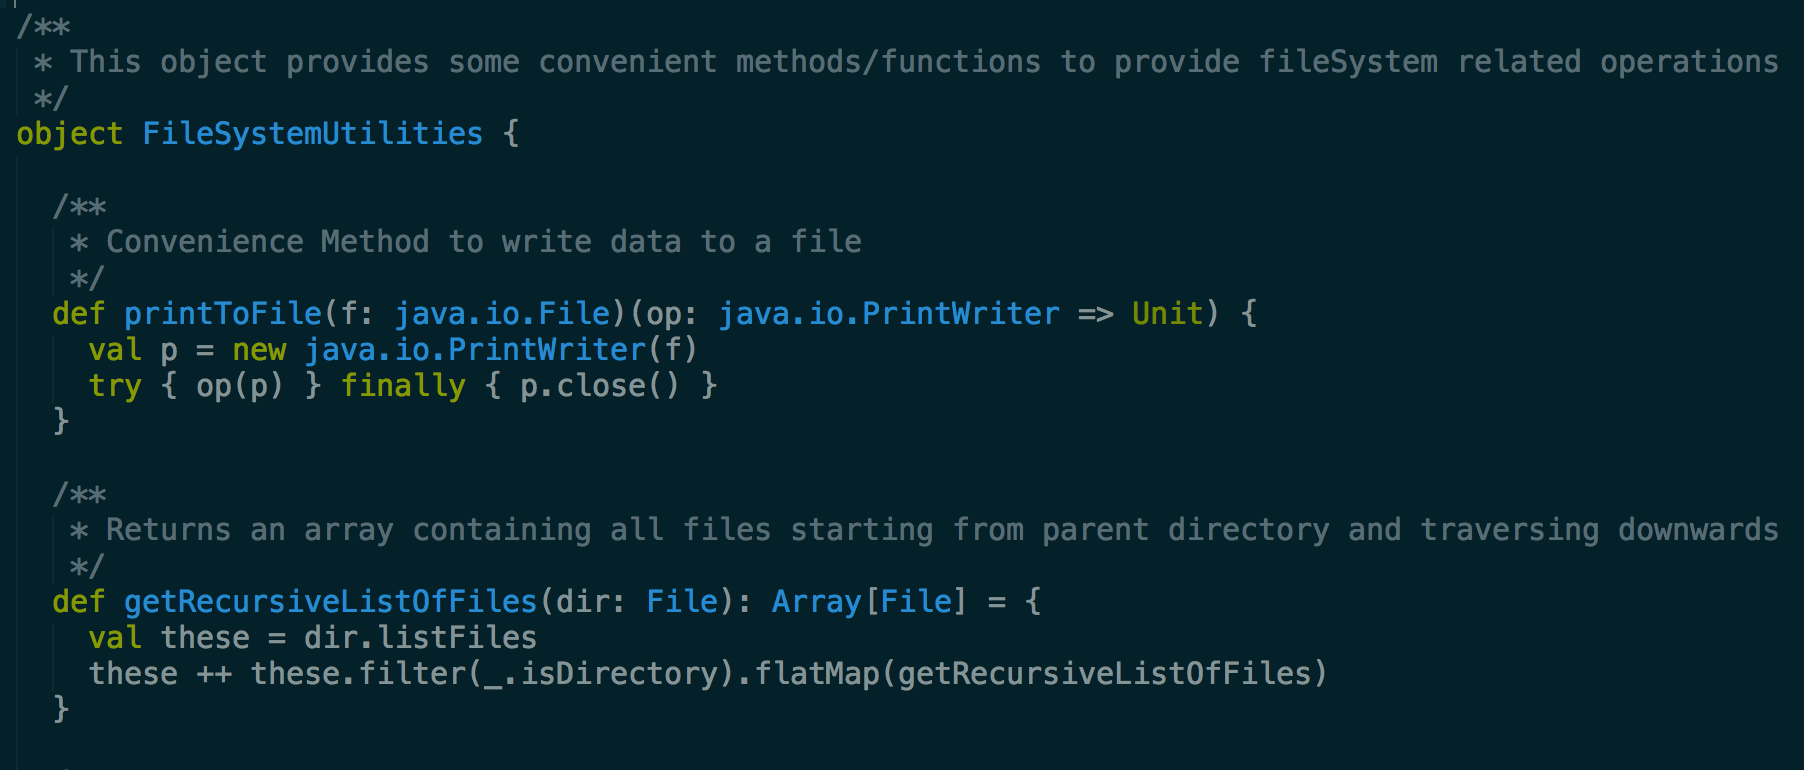
\includegraphics[width=400px]{figures/singleton.png}
  \caption{An example of Singleton pattern usage}
\end{figure}

\noindent
\textbf{Explanation} - The example above is straightforward. The methods inside the object can be directly accessed by invoking \textless object\_name \textgreater.\textless method\_name(args) \textgreater. Scala \textit{objects} also provide a great way to have singleton implementations of traits.
For example, creation of thread - safe methods require an extension of the trait \textbf{Runnable}. Methods can be implemented without considering factors like thread - safety and multiple instantiations.

\begin{figure}[H]
  \centering
    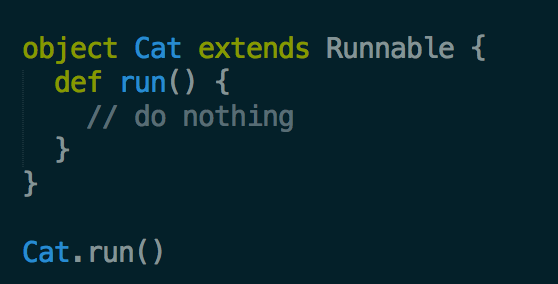
\includegraphics[width=300px]{figures/singleton2.png}
  \caption{An example of Singleton pattern usage}
\end{figure}

\noindent
The reasons for choosing the \textit{Singleton} pattern were:
\begin{itemize}
\item Lazy initialization leading to optimized heap memory usage
\item Concise Syntax
\item Thread Safety
\item Clear Intent
\end{itemize}

% Explanation of Builder Pattern
\subsubsection{Builder Pattern}
Builder pattern builds a complex object using simple objects and using a step by step approach. This type of design pattern comes under creational patterns as this pattern provides one of the best ways to create an object. Our SLEEK/HIP tests are instantiated incrementally and therefore the builder pattern is natural choice. The builder pattern combined with the \textbf{fluent interface} concept gives the DSL a declarative feel.
\bigskip

\noindent
Fowler's concept of the "Fluent Interface" can be extended to Scala which models behaviour using traits rather than interfaces \cite{scala}. This in conjunction with the builder pattern lead to a declarative syntax. One of the uses of the builder is shown below.

\begin{figure}[H]
  \centering
    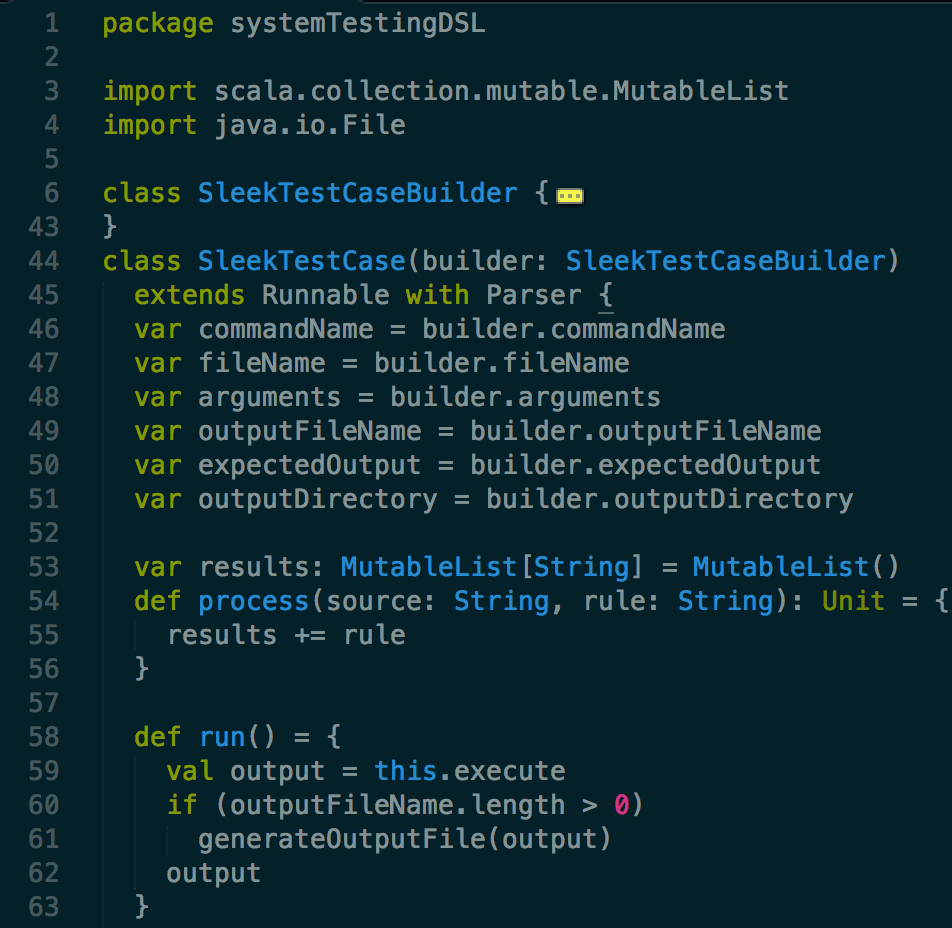
\includegraphics[width=400px]{figures/builder_pattern.png}
  \caption{An example of builder pattern usage}
\end{figure}

\noindent
The reasons for choosing the \textit{Builder} pattern were:
\begin{itemize}
\item Natural language like syntax enhancing readability
\item Logic is built into the syntax
\item The parameters being provided to the base type can be provided in different stages as the builder manages the object instantiation.
\end{itemize}

% Explanation of Factory Pattern
\subsubsection{Factory Pattern}
This is used in the project by defining trait for creating an object, but let the classes that implement the interface decide which class to instantiate. The Factory method lets a class defer instantiation to subclasses. For context - aware choice of which kind of class to instantiate. This has been used to switch between \textbf{Console Output and HTML Output}.

\begin{figure}[H]
  \centering
    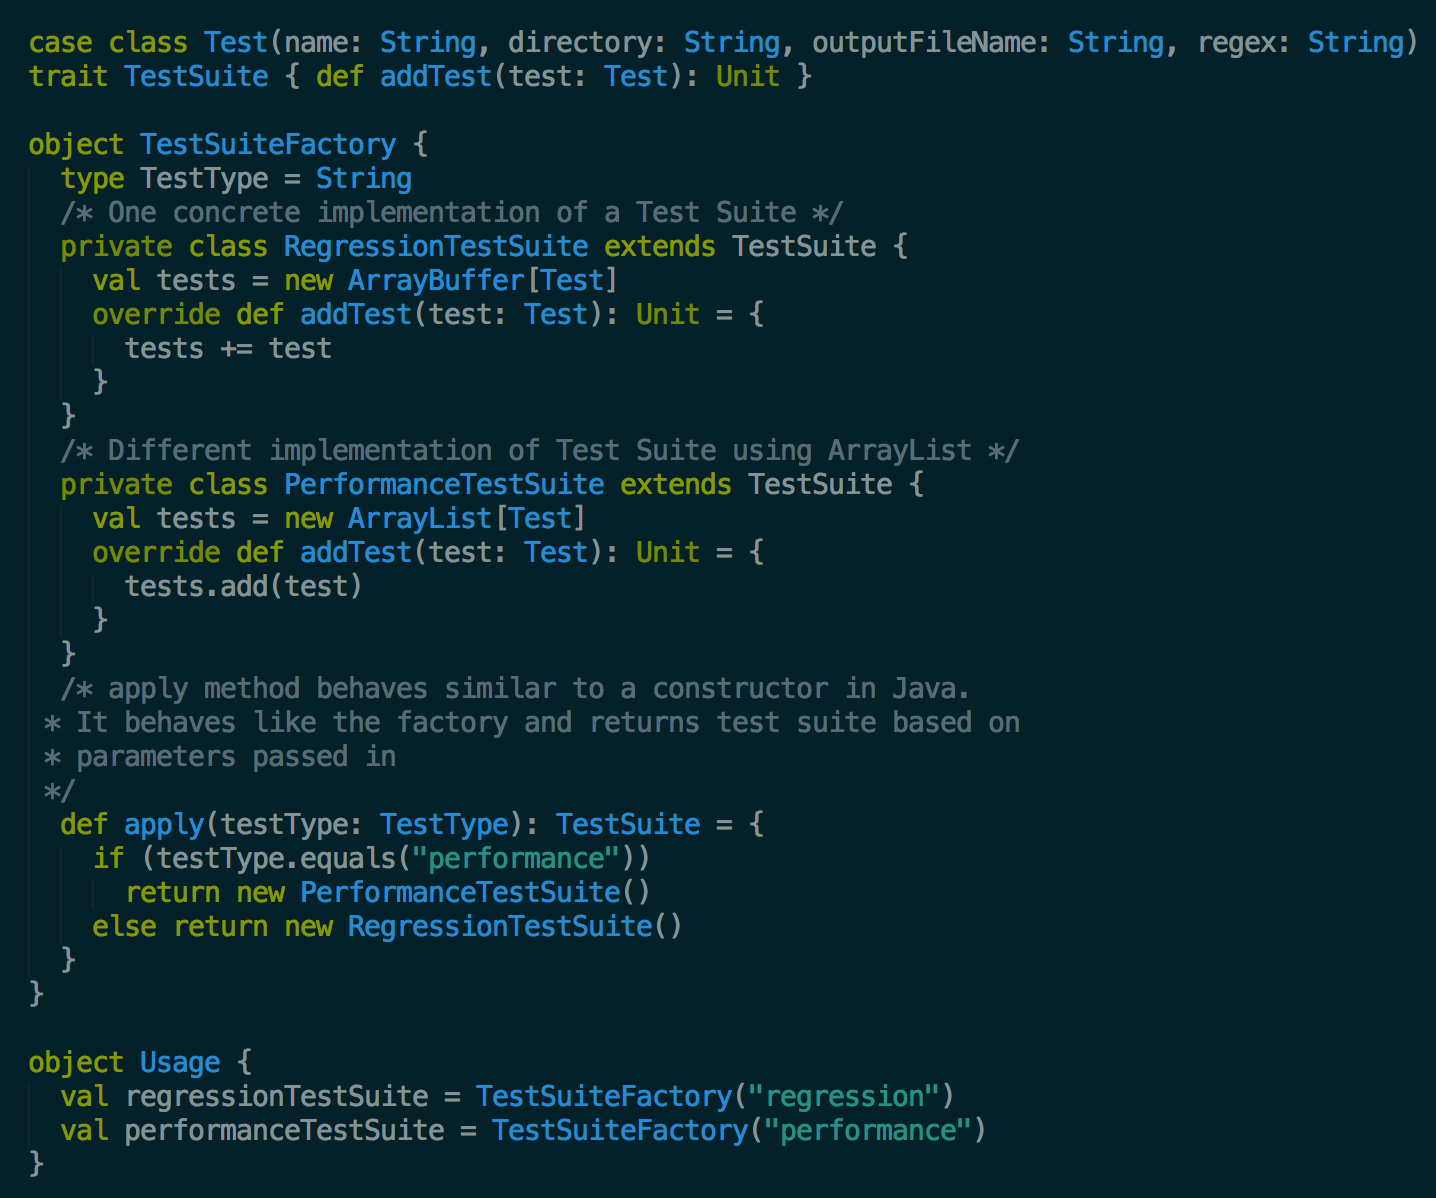
\includegraphics[width=500px]{figures/factory.png}
    \caption{An example of how Factory Pattern is used}
\end{figure}

\noindent
\textbf{Explanation} - The trait \textbf{TestSuite} specifies certain methods that any test suite must implement. Two concrete implementations of \textbf{TestSuite} are \textbf{RegressionTestSuite} and \textbf{PerformanceTestSuite}. The companion object, \textbf{TestSuite} implements the \textbf{Factory Pattern} by deciding which kind of TestSuite to instantiate - the RegressionTestSuite or PerformanceTestSuite based on some input parameters. For the sake of simplicity, here a string type parameter has been shown. However, in the application code, a \textbf{Configuration} type has been passed in as the parameter.

\noindent
The reasons for choosing the \textit{Factory} pattern were:
\begin{itemize}
\item Better abstraction
\item Internal implementation details are not revealed to clients
\item Stronger inheritance relationship
\end{itemize}

% Explanation of Future Timeout
\subsubsection{Future Timeout Design Pattern}
Scala Futures provide an elegant way of handling asynchronous operations in Scala \cite{scala}. They allow developers to write non - blocking processes running on a different thread. They allow us to wait on the thread for completion (which is actually an anti - pattern because we could have just used a blocking call), pass messages/arguments to the thread when it is done executing (\textit{Promises}) or just time - out after a certain duration (\textit{Awaits}). In this context, the time - out pattern using Awaits is being used to prevent processes from blocking indefinitely. This can be set by setting the \textbf{TIMEOUT} variable in the system configuration.

\begin{figure}[H]
  \centering
    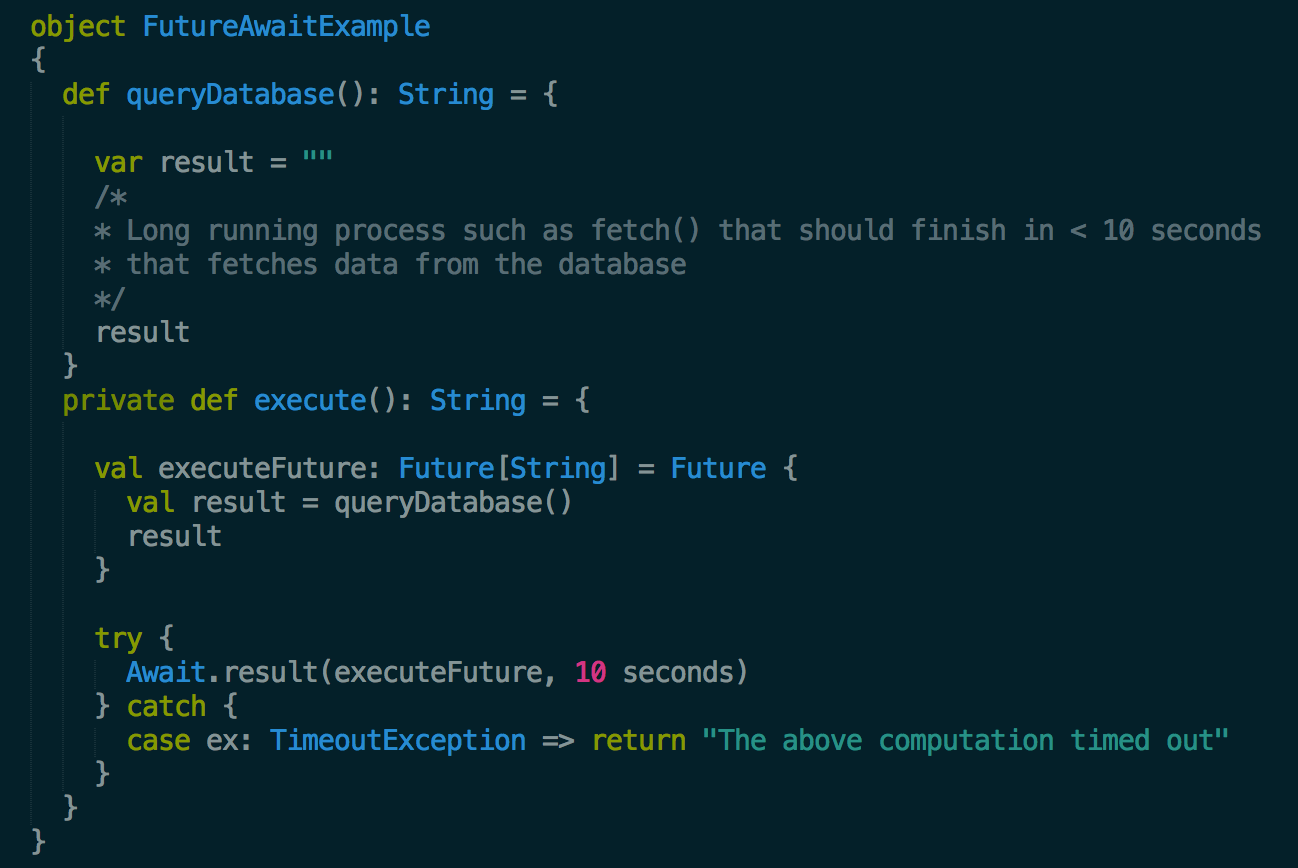
\includegraphics[width=500px]{figures/future_timeout.png}
  \caption{An example of "Future Timeout" pattern usage}
\end{figure}

\noindent
\textbf{Explanation} - The future timeout pattern is specific to languages like Scala that provide concurrent constructs such as \textbf{Futures}, \textbf{Promises} and \textbf{Awaits}. In the above example, the function call that takes a substantial amount of time is the queryDatabase() method, which is supposed to return a \textit{string} value. Scala allows us to wrap it in a \textbf{Future} block. It's return type therefore becomes a \textbf{Future[String]}. The \textbf{Await} construct allows to wait on the Future for a specified time period (in this case 10 seconds). If the computation takes longer, an exception is thrown and dealt with appropriately inside the catch block.

\noindent
The reasons for choosing the \textit{Future - Timeout} pattern were:
\begin{itemize}
\item Concise syntax
\item Logic is built into the syntax
\item Abstracts lower level threading details
\end{itemize}
% Explanation of Dependency Injection
\subsubsection{Dependency Injection (DI) Pattern}

This pattern allows developers to avoid hard-coded dependencies and to substitute dependencies either at run-time or at compile time. It is a special case of the Inversion of Control (IoC) pattern. It also allows us to choose between multiple implementations of a particular component in an application\cite{gof}. DI has been applied throughout the project to reduce coupling and make the code as extensible as possible. For example, \textbf{constructor injection} is performed for configuration type objects where custom configurations are possible.

\begin{figure}[H]
  \centering
    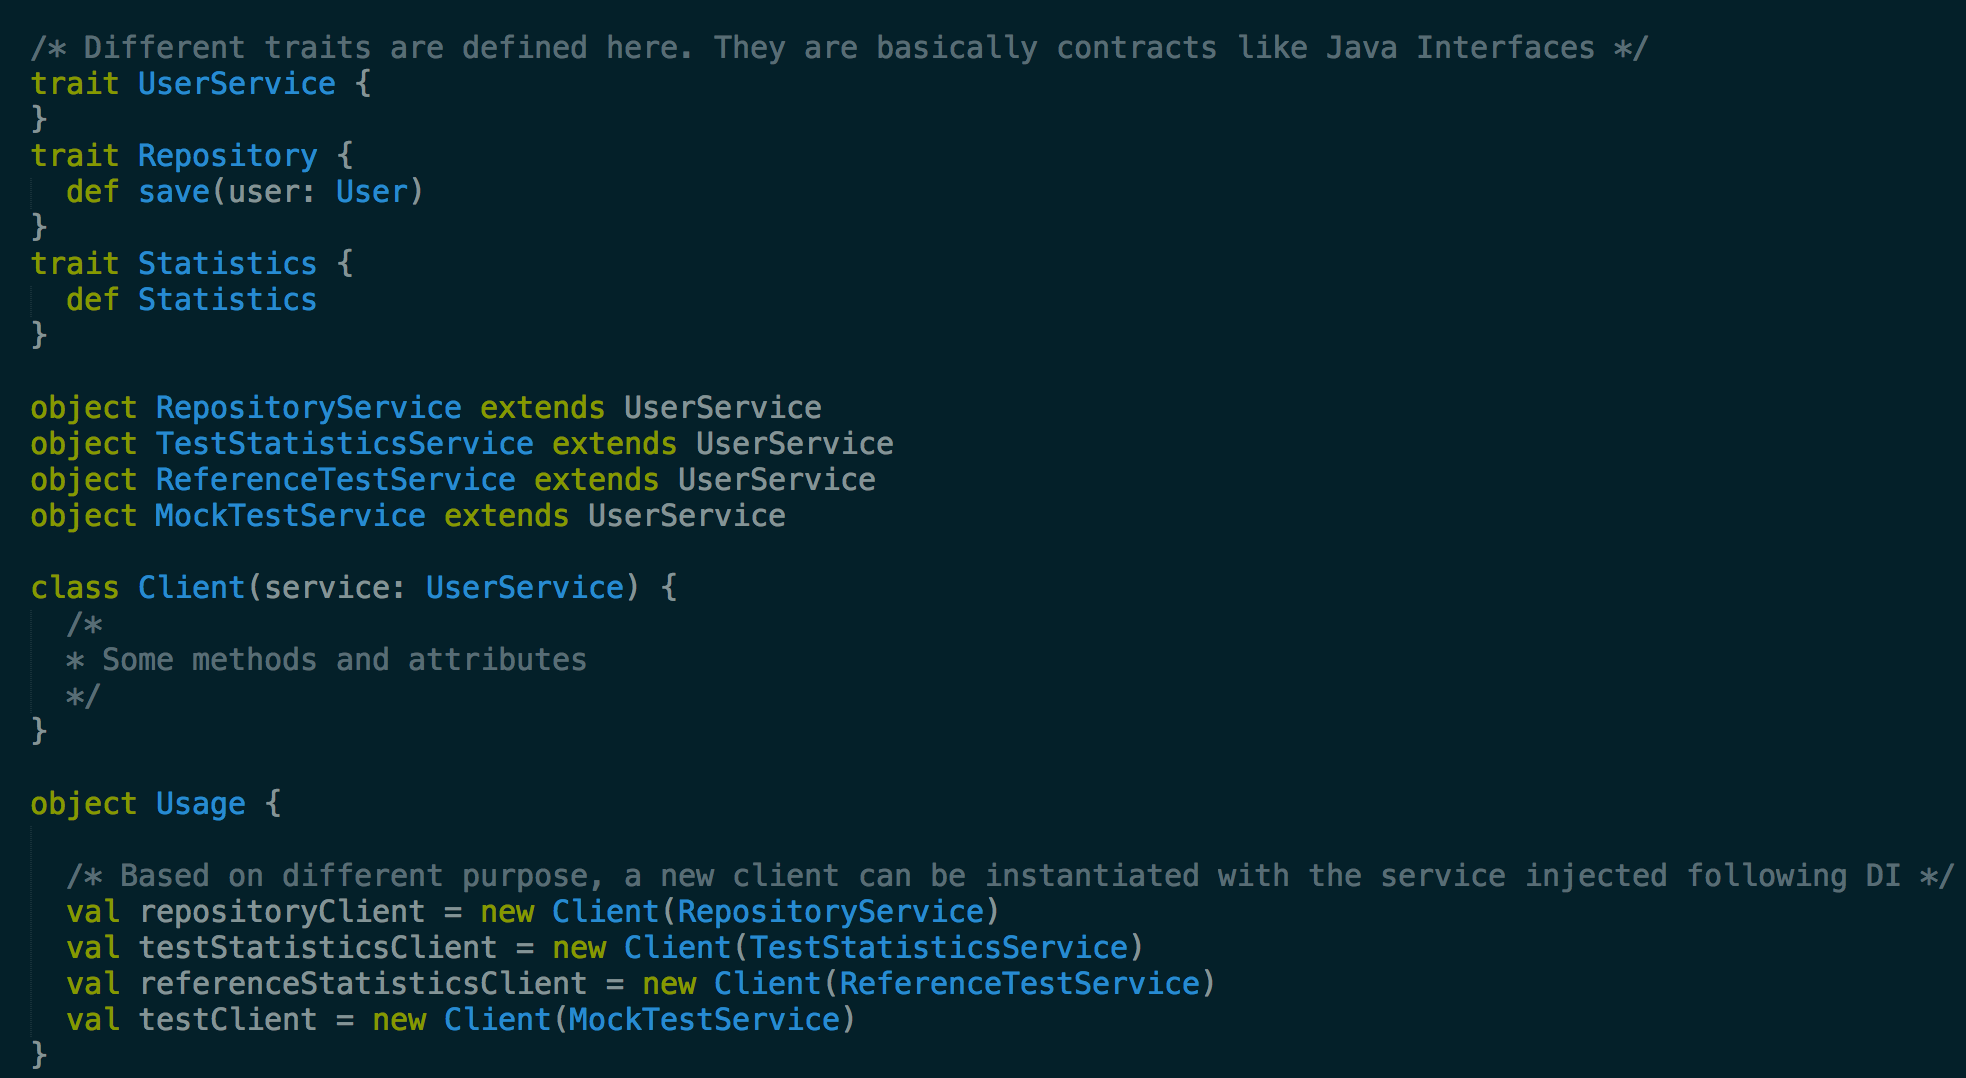
\includegraphics[width=520px]{figures/di.png}
  \caption{An example of how DI is used}
\end{figure}
\noindent

\noindent
\textbf{Explanation}: The DI pattern has been used in several places throughout the project to facilitate ease of testing, multiple implementation support and general loosely coupled design. In the code skeleton above, the \textbf{UserService} trait specifies certain behaviour (like a Java Interface). Some of the concrete implementations of these behaviours are the \textbf{RepositoryService, TestStatisticsService, ReferenceTestService}. The \textbf{MockTestService} is just a drop-in that can be used for unit testing the code. The type Client requires an \textbf{UserService} as a dependency. We can just inject in concrete implementations of the Services based on the kind of Client we are instantiating. This is a simplified example of how DI has been used in the project.
\bigskip

\noindent
The reasons for choosing the \textit{Dependency Injection} pattern were:
\begin{itemize}
\item Loose coupling leading to extensibility
\item Static checking of dependencies (unlike XML based DI implementations)
\item Concise syntax
\end{itemize}
\subsection{Configuration Media}

The DSLs developed require configuration in a human - readable format so that developers can conveniently integrate them into the testing work - flow. To keep both DSLs decoupled, they each have a configuration file. They can be configured by using YAML markup.  YAML, or "YAML Ain't Markup Language", is "a human friendly data serialization standard for all programming languages."
\bigskip

\noindent
\textbf{Configuring the Scala DSL} - The \textit{application.conf} file contains settings specific to the HIP/SLEEK verification systems, regression test construction and regression test execution. Some general system level settings such as output file extensions and time - outs are also specified.
\bigskip

\noindent
It is important to note that friendliness and readability are primary strengths of YAML. The number of format characters is very low and, like Python, YAML's markup can use whitespace characters to indicate scope. Tabs are not permitted inside YAML and any YAML parser will throw errors and indicate that the file is not well - formed YAML \cite{yaml}. YAML's internal data structures like sequences, maps and objects are very much like those of dynamic languages like Python and Ruby. An example of YAML markup is shown below:

\begin{figure}[H]
  \centering
    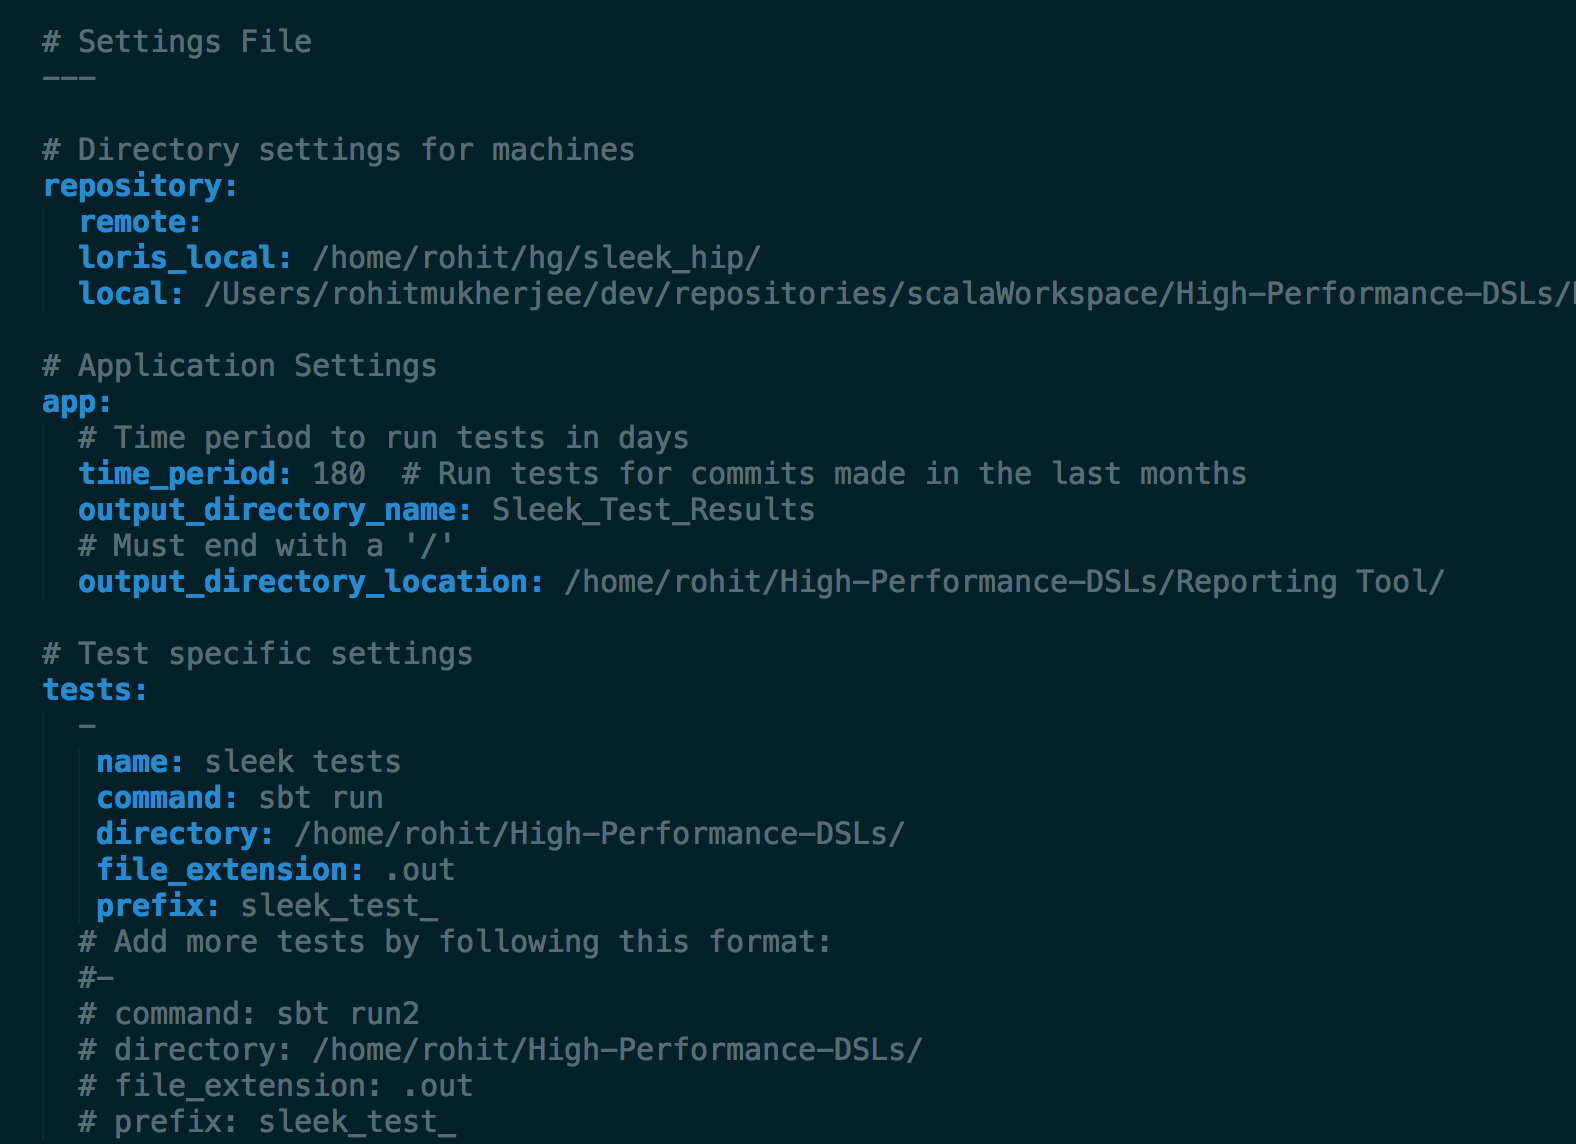
\includegraphics[width=400px]{figures/settings.png}
  \caption{settings.yaml - used to configure the reporting tool}
\end{figure}

\noindent
\textbf{Explanation} - The repository object contains the attributes remote and local. It also contains application specific settings such as time period and output directory name and location. The reasons for using YAML are:
\begin{itemize}
\item Human Readability
\item Low number of format characters
\item Language agnostic, can be parsed easily by different languages
\item Sufficient types of data structures
\item Not verbose like XML
\item Faster than XML
\item Pythonic syntax
\end{itemize}

% Deployment and Build Choices %
\subsection{Deployment/Build Choices}
The entire project is managed using \textbf{Simple Build Tool} or \textbf{SBT}. SBT is itself a DSL and interactive build tool which supports parallel running of tests/build tasks. The following options are supported by the system \cite{sbt}. \textbf{SBT} is an open - source build tool for \textbf{Scala} and \textbf{Java} projects, similar to Java's \textbf{Maven }or \textbf{Ant} or \textbf{GNU Make} for C and C++. \textbf{SBT} is the \textit{de facto} build tool for the Scala community.
\bigskip

\noindent
The company that produces Scala, Typesafe recommends sbt as the best tool for building and maintaining Scala projects. Some of the key features because of which sbt was used during this project are as follows:
\begin{itemize}
\item Incremental compilation - The whole project does not need to be recompiled, new byte - code is generated from files that have changed since last compilation
\item Interactive Shell - Easy to use and convenient to debug
\item Native support for compiling Scala code and integrating with many Scala test frameworks
\item Build descriptions written in a Scala DSL\cite{sbt}
\item Dependency management and plugin management (similar to Maven)
\end{itemize}
 
The build configuration file \textbf{build.sbt} used in the project is shown below:

\begin{figure}[H]
  \centering
    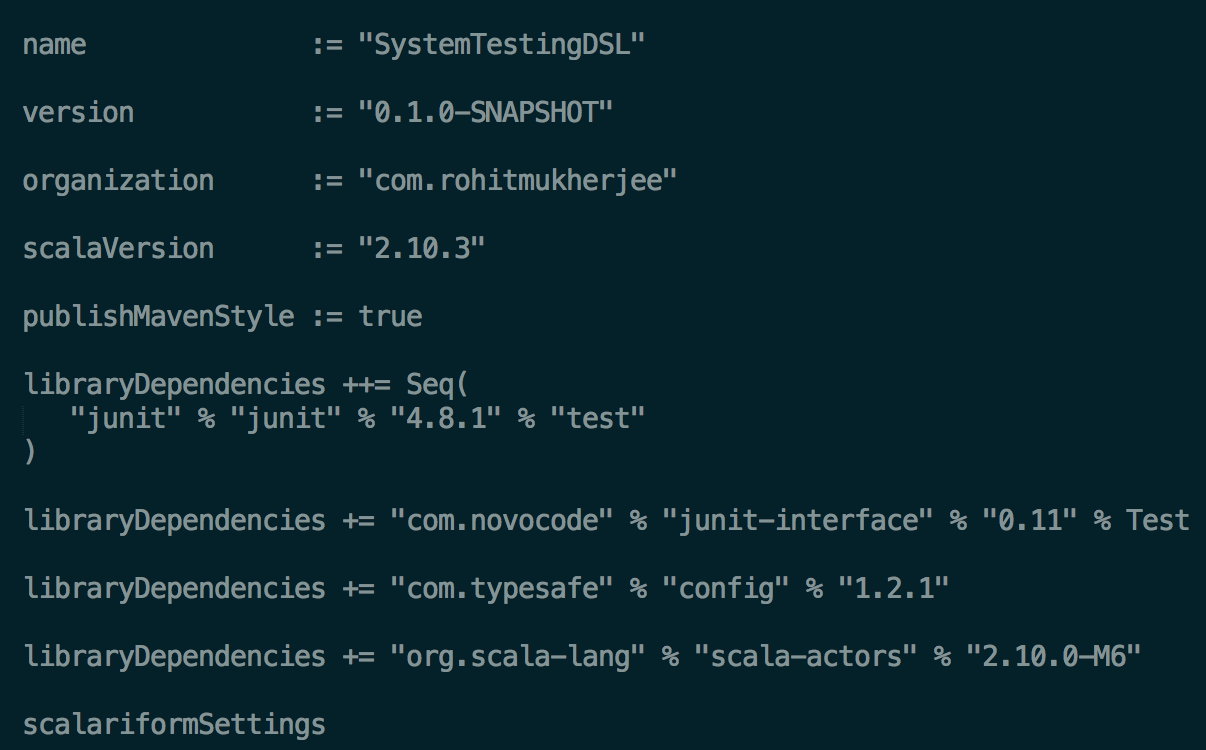
\includegraphics[width=500px]{figures/build_sbt.png}
  \caption{build.sbt - Build file to manage project}
\end{figure}

\noindent
The above build file mentions project name, version information, publisher name and dependencies the project has such as \textbf{scalariform} for formatting source code, \textbf{JUnit} for unit testing and \textbf{Typesafe Config} for configuration via dependency injection.
\bigskip

\noindent
The project supports several build targets for running different kinds of tests such as HIP/SLEEK, performance and regression tests. These targets can be changed or extended by editing the \textbf{src/main/scala/systemTestingDSL/Main.scala}. The targets supported are:
\begin{itemize}
\item \textbf{sbt "run sleek"} - Executes all sleek tests
\item \textbf{sbt "run hip"} - Executes all hip tests
\item \textbf{sbt "run buildReference"} - Constructs references for regression testing
\item \textbf{sbt "run runReference"} - Runs tests against constructed references
\item \textbf{sbt "run overrideReference"} - Re - processes references
\item \textbf{sbt "run test"} - Executes unit tests written during development process.
\item \textbf{sbt "run help"} - Shows supported operations
\end{itemize}
\newpage